\section{Active Learning} \label{sect:theory:active-learning}

Active learning is a paradigm in which a system attempts to learn the label of an observation by enabling users (or other sources) catalog unlabeled observations \cite{report:active-learning}. By doing this, the model aims to learn the relationship among the observations and their labels using as few observations as possible. Active learning seeks to overcome the labelling bottleneck, specially when there is a large amount of unlabeled data or when obtaining such labels is expensive \cite{report:active-learning}. Figure \ref{fig:active-learning} shows an example active learning setup, where a user(s) is in charge of labeling data.

\begin{figure}[H]
  \centering
  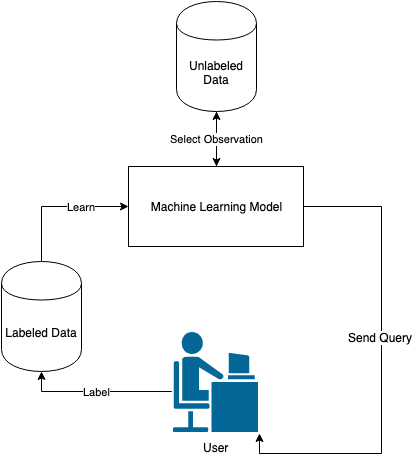
\includegraphics[
        width=\textwidth,
        height=0.4\textheight,
        keepaspectratio
  ]{report/images/active-learning.png}
  \caption{Diagram illustration of a possible active learning setup which relies in a user to label data.}
  \label{fig:active-learning}
\end{figure}